\chapter{Side projects}

\section{Healthcare Network}

\section{Affiliation Generator}

Affiliation Generator is a web application that helps you manage your papers authors and their affiliations. The app will let you upload a list of researchers from your team, as well as their affiliations. When you're writing a new paper, simply drag and drop authors in the required order of authorship and the app will generate the list of authors to copy-paste in your paper.

You can edit your researchers and institutions list. Every researcher can be attached to one or many institutions. The generator page will let you drag and drop researchers in the order of authorship on your paper. Once your click generate, the app will retrieve the affiliations from your researchers and format them automatically for you so that you only have to copy paste this into your paper. You can also create papers, drag and drop the authors in the order you want, save them and add more authors later.

The application is deployed within Institut Curie at the following address:

\url{https://affiliation-generator.curie.net/}.

\begin{figure}[h]
    \includegraphics[width=0.7\textwidth]{images/healthcare-network/home.png}
    \centering
    \caption{}
    \label{fig:hn-home}
\end{figure}


\begin{figure}[h]
    \includegraphics[width=0.7\textwidth]{images/healthcare-network/search.png}
    \centering
    \caption{}
    \label{fig:hn-search}
\end{figure}


\begin{figure}[h]
    \includegraphics[width=0.7\textwidth]{images/healthcare-network/curie-services.png}
    \centering
    \caption{}
    \label{fig:hn-curie-services}
\end{figure}


\begin{figure}[h]
    \includegraphics[width=0.7\textwidth]{images/healthcare-network/curie-cancero.png}
    \centering
    \caption{}
    \label{fig:hn-curie-cancero}
\end{figure}


\begin{figure}[h]
    \includegraphics[width=0.7\textwidth]{images/healthcare-network/curie-dp.png}
    \centering
    \caption{}
    \label{fig:hn-curie-dp}
\end{figure}


\begin{figure}[h]
    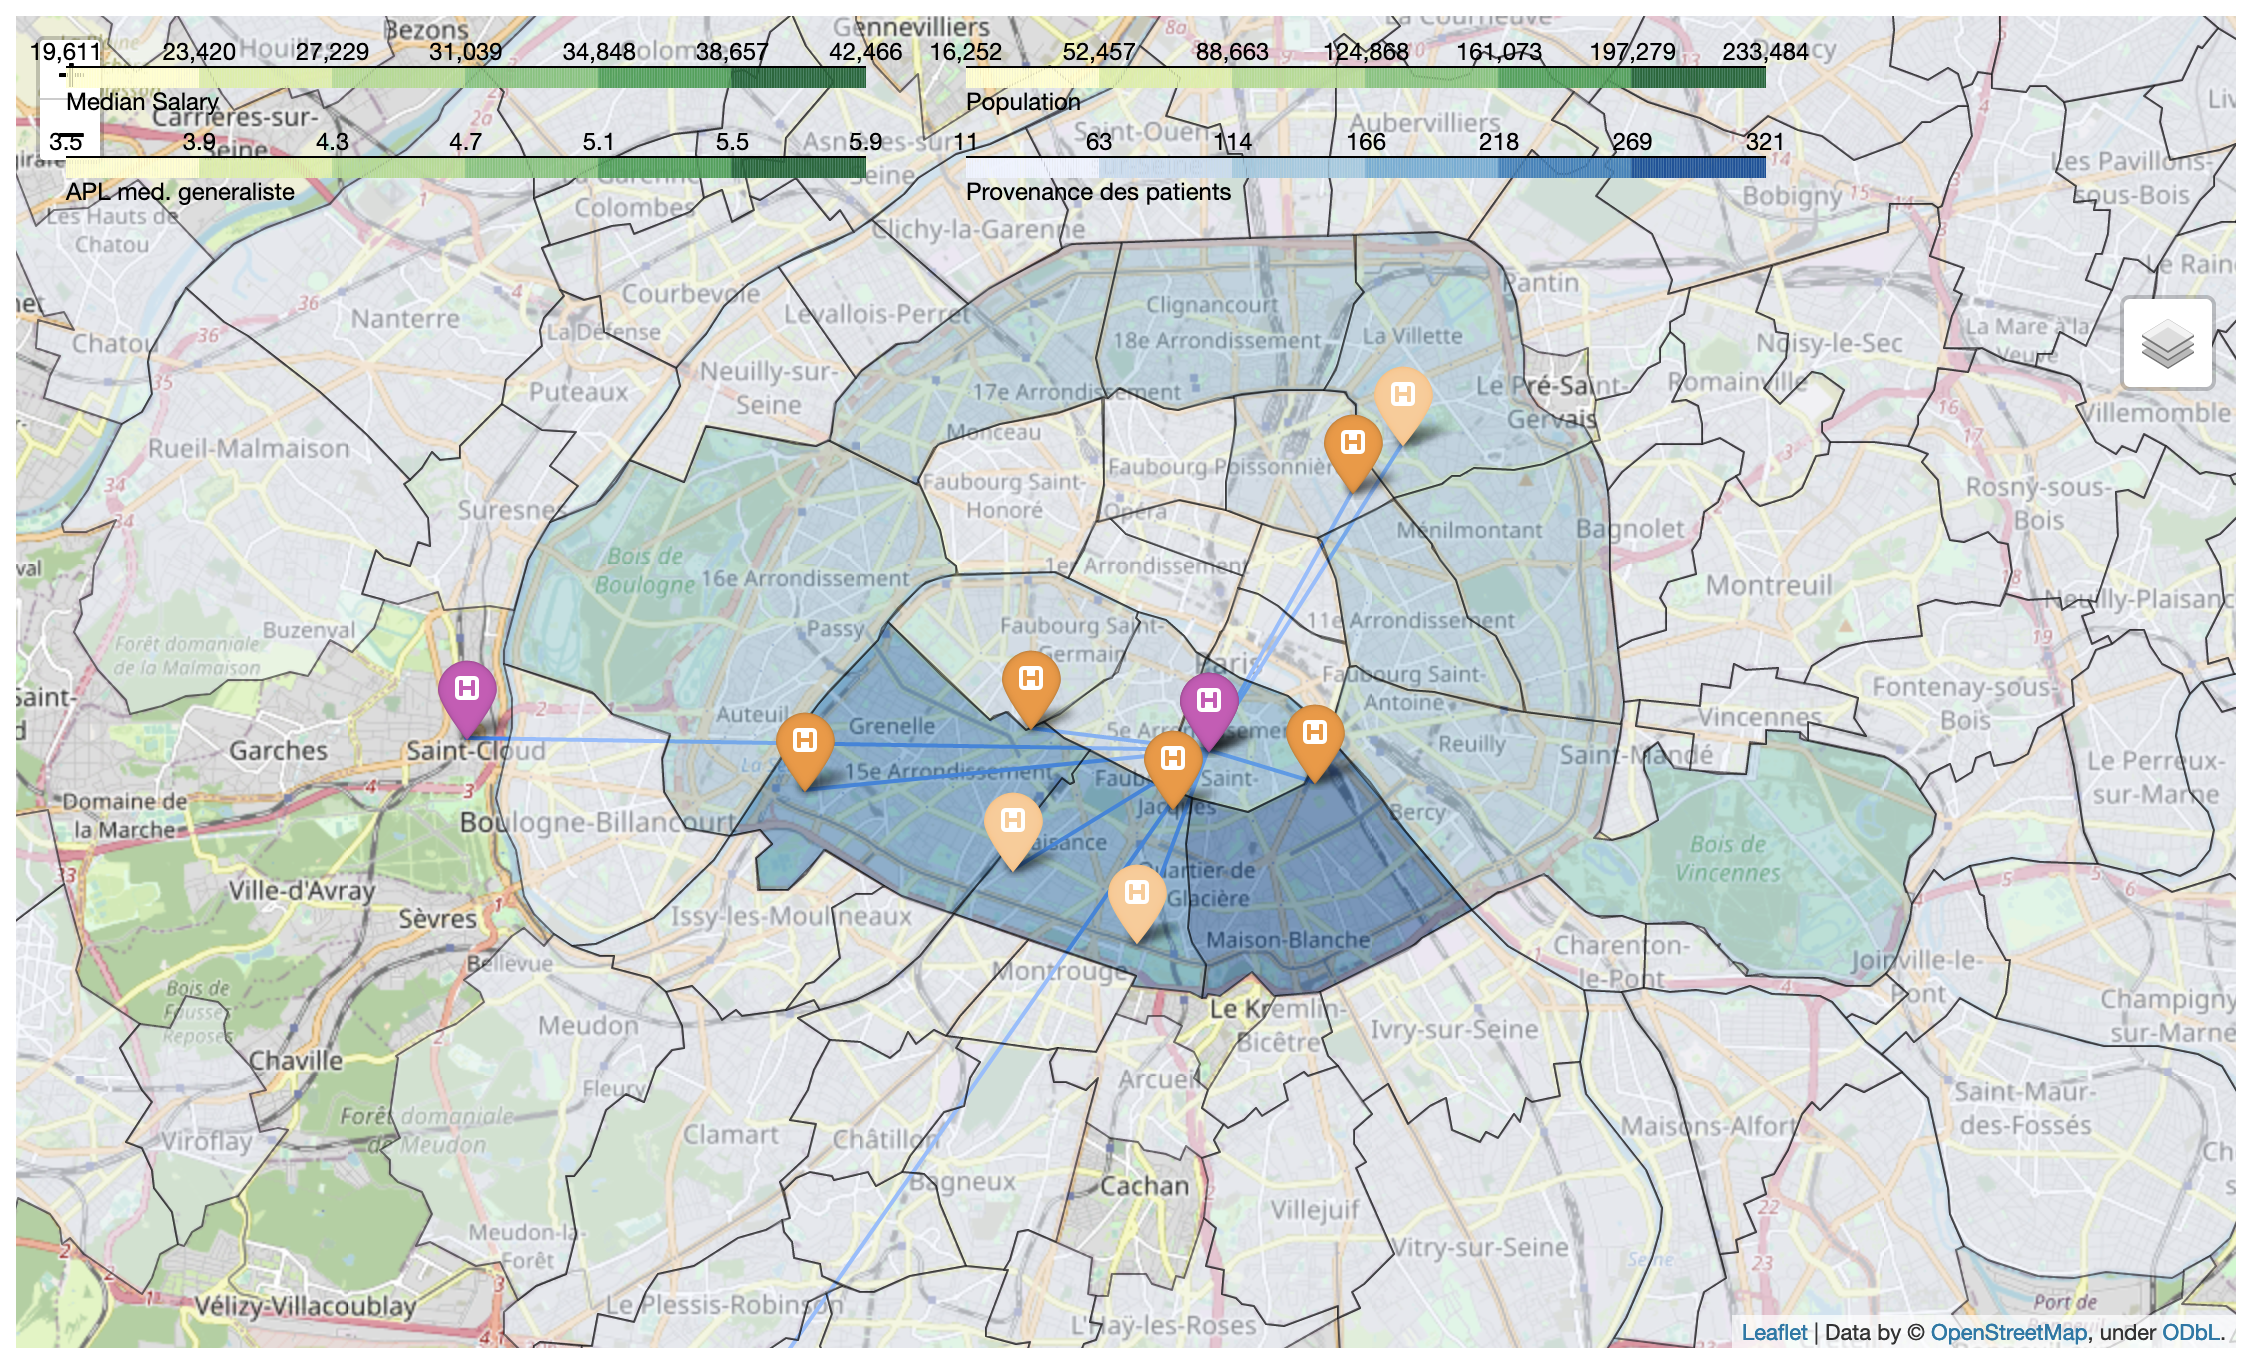
\includegraphics[width=0.7\textwidth]{images/healthcare-network/curie-co-occ.png}
    \centering
    \caption{}
    \label{fig:hn-curie-co-occ}
\end{figure}


\begin{figure}[h]
    \includegraphics[width=0.7\textwidth]{images/healthcare-network/curie-commune.png}
    \centering
    \caption{}
    \label{fig:hn-curie-commune}
\end{figure}
